\section{测试、运行情况}

\subsection{大雾实验工具}

本程序的每一个实验模块由组员完成后,组长会进行代码审核与测试,
如果发现问题则要求继续修改,直到所有问题被解决后该实验模块才会发布。

另一方面,各种 API 的编写与模块化编程也让我们的程序在编写过程中更不容易出错,
同时规范、统一的码风也让调试变得轻松。

% \begin{figure}[htbp]
%   \centering
%   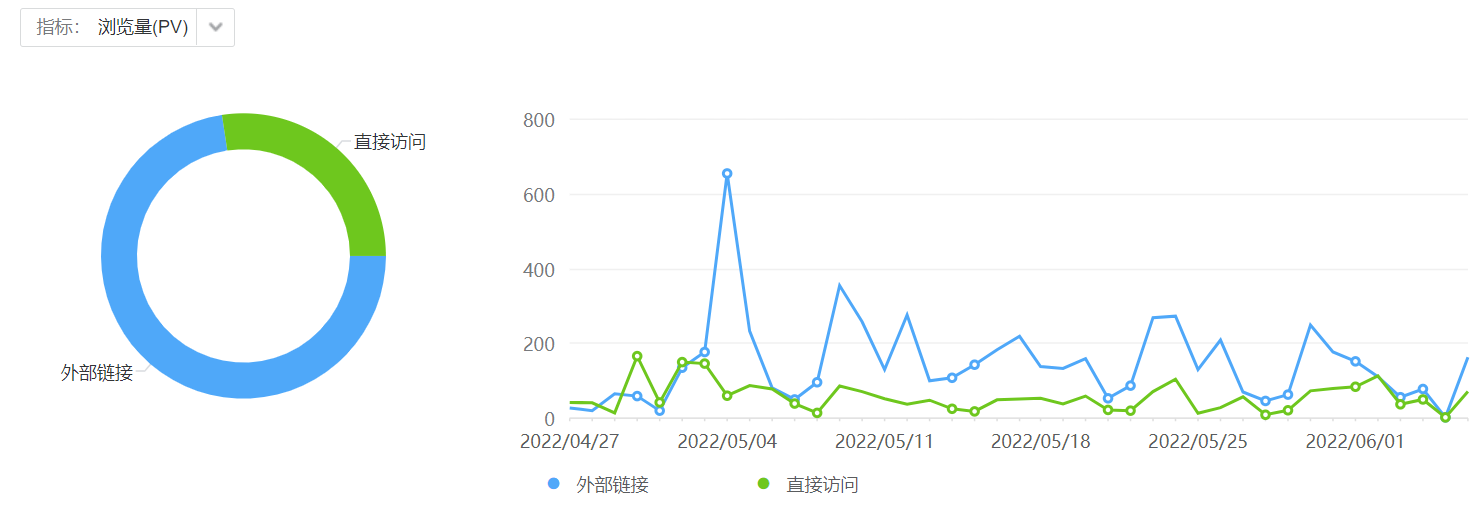
\includegraphics[width=\columnwidth]{figure/0.png}
%   \caption{4 月 27 日至 6 月 7 日的网站浏览量}
%   \label{fig:0}
% \end{figure}
% \begin{figure}[htbp]
%   \centering
%   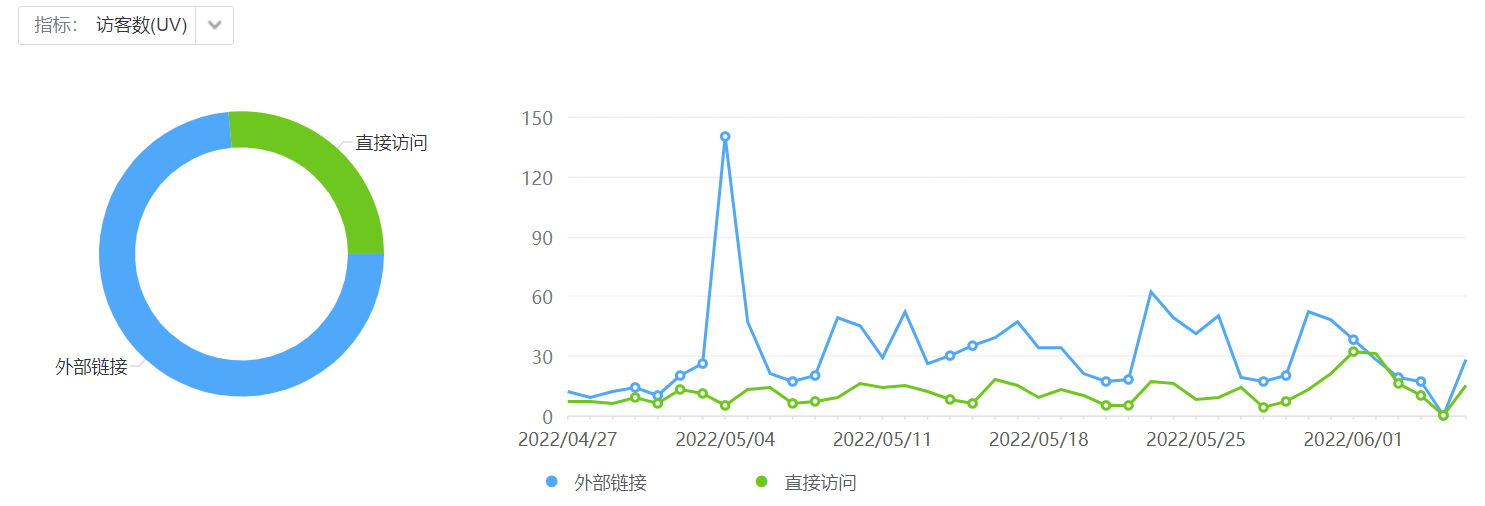
\includegraphics[width=\columnwidth]{figure/1.png}
%   \caption{4 月 27 日至 6 月 7 日的网站访客数}
%   \label{fig:1}
% \end{figure}

网站的访问统计如图 \ref{fig:2} 所示,可以看出我们的工具有 800 多名稳定用户,日均浏览量超过2300人次。
同时,本工具在 GitHub 上开源,同学们可以进一步完善其功能。

\begin{figure}[htbp]
  \centering
  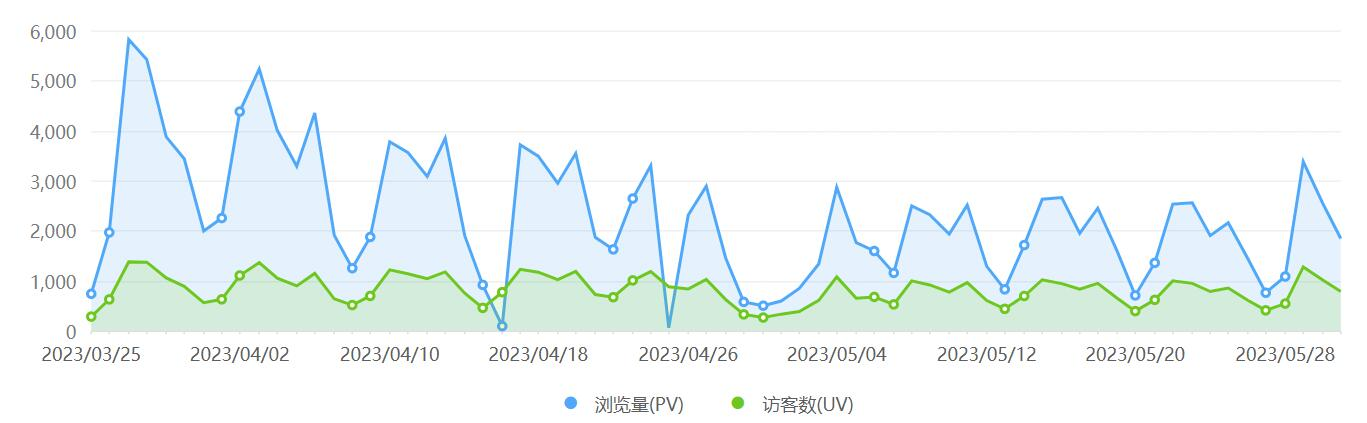
\includegraphics[width=\columnwidth]{figure/2.jpg}
  \caption{大雾实验工具运行情况(2023春季学期)}
  \label{fig:2}
\end{figure}

\subsection{蜗壳排课工具}

蜗壳排课工具的开发完成时间较晚,于本学期开始前刚刚发布。但根据统计数据,本学期选课周的日浏览量峰值已经接近 2000 人次(如图 \ref{fig:3} 所示),可见该工具具有光明的前景。

\begin{figure}[htbp]
  \centering
  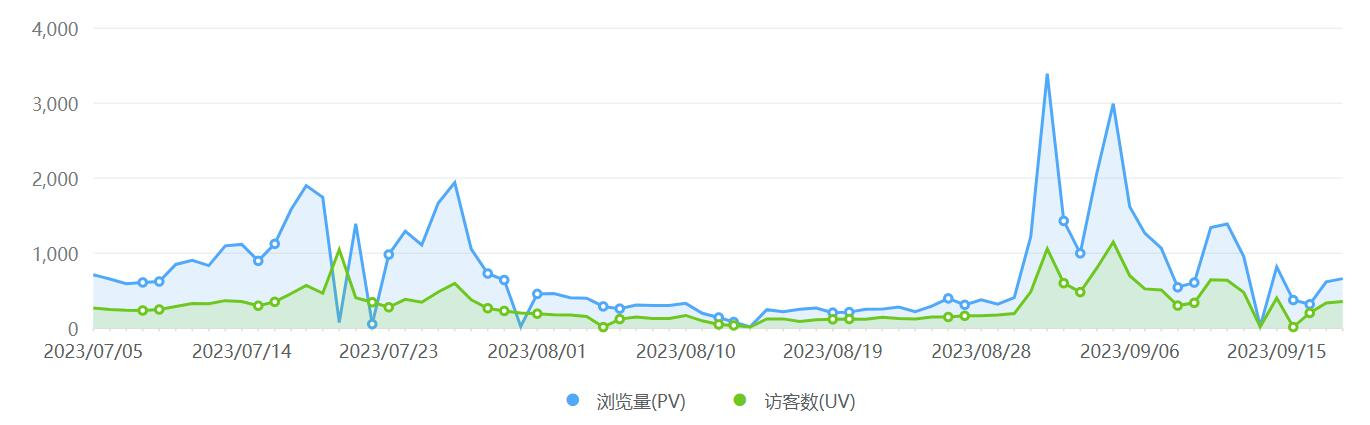
\includegraphics[width=\columnwidth]{figure/3.jpg}
  \caption{蜗壳排课工具运行情况(2023年7--9月)}
  \label{fig:3}
\end{figure}

\subsection{我的科大APP}

尽管APP的推广之路充满了挑战,但至今,我的科大APP已经拥有超过 5000 名用户(如图 \ref{fig:4} 所示),仅在八月份就新增了超过 1200 名用户,这些用户主要为大一新生,考虑到本APP仅提供了安卓版,可见其市场占有率非常之高。我们每日活跃用户达到 2000 人(如图 \ref{fig:5} 所示,其中10月初有一个曲线谷是因为国庆假期),每日启动次数约为 20000 人次。这些数据充分反映了我们的产品受到了用户的热烈欢迎。

\begin{figure}[htbp]
  \centering
  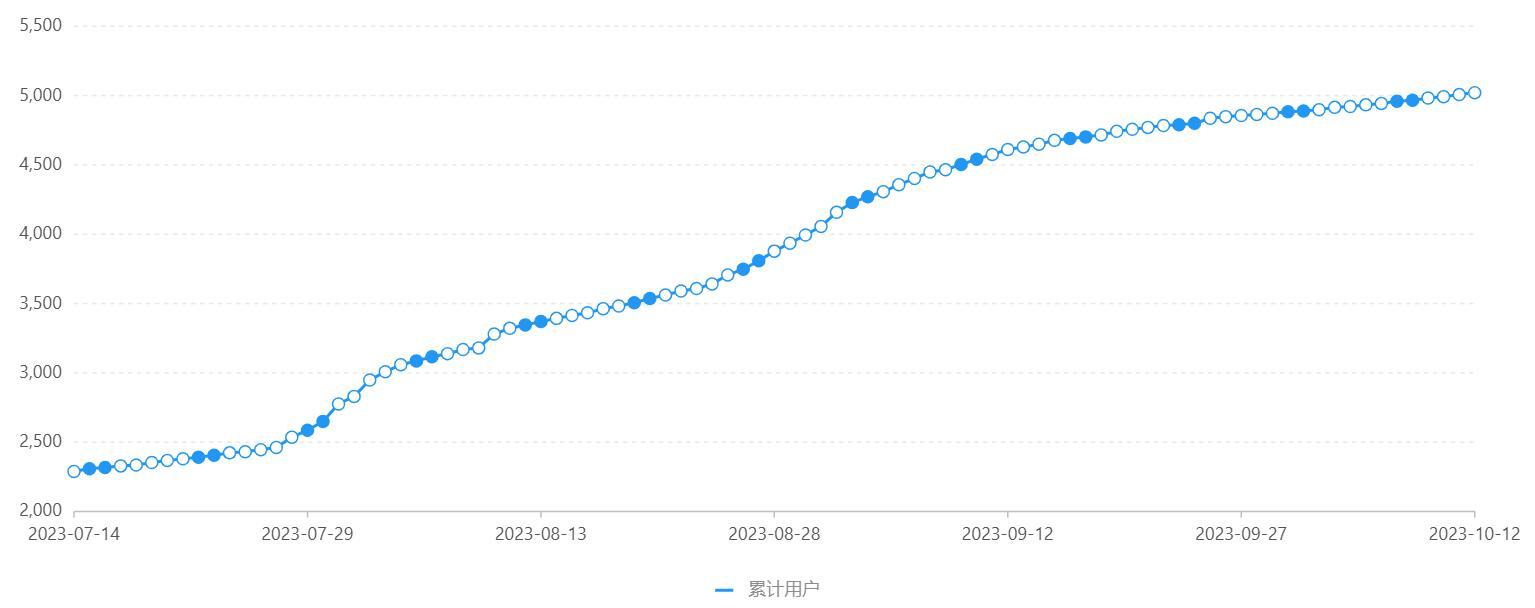
\includegraphics[width=\columnwidth]{figure/4.jpg}
  \caption{我的科大APP累计用户(2023年7--10月)}
  \label{fig:4}
\end{figure}

\begin{figure}[htbp]
  \centering
  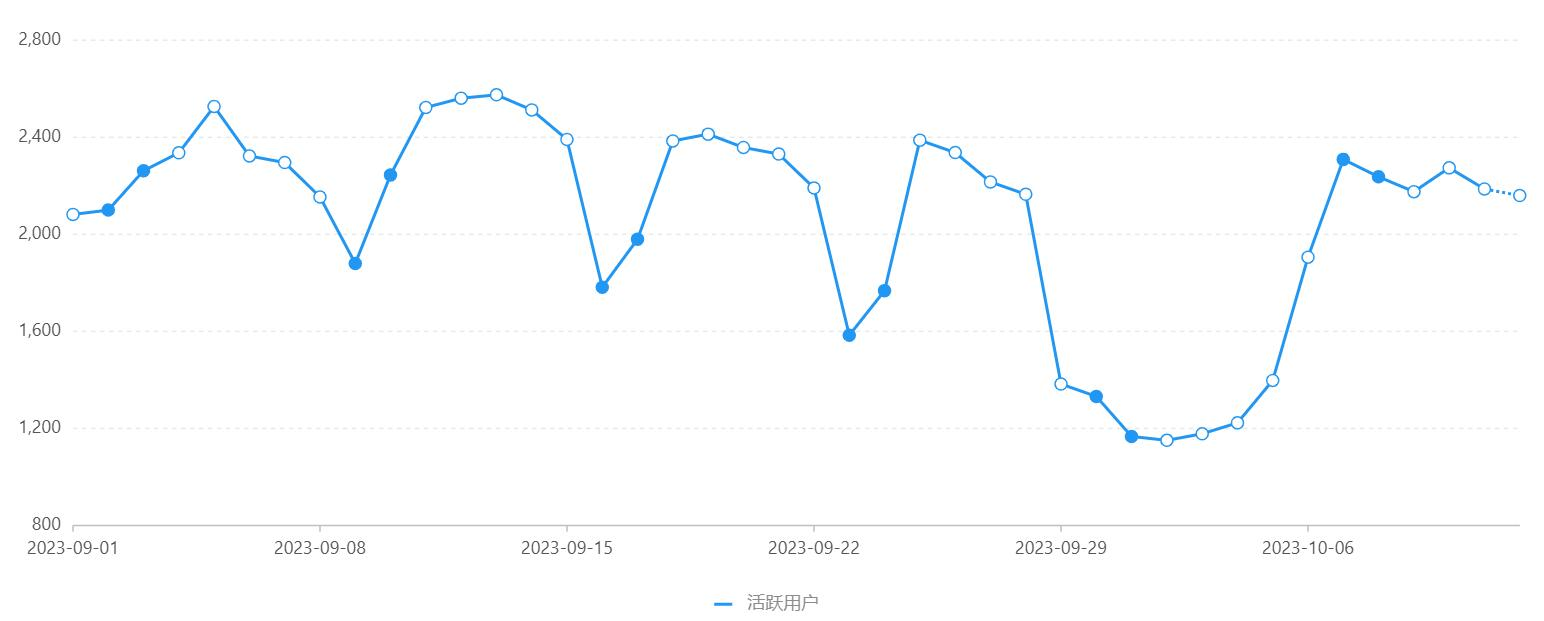
\includegraphics[width=\columnwidth]{figure/5.jpg}
  \caption{我的科大APP活跃用户(2023年9--10月)}
  \label{fig:5}
\end{figure}